\section*{Outline}
%%%%%%%%%%%%%%%%%%%%%%%%%%%%%%%%%%%%%%%%%%%%%%%%%%%%%%%%%%%%%%%%%%%%
\begin{frame}
  \frametitle{Learning Goals}
    \begin{itemize}
        \item Implementation of a non-trivial project in a small group as well as an individual extension of it.
        \item Get a feeling for intra- and inter-node parallelization strategies and frameworks.
        \item Usage of established frameworks in the High-Performance Computing (HPC) community like \link{https://www.openmp.org/}{OpenMP} and \link{https://www.mpi-forum.org/}{MPI}.
        \item Practical application of tree data structures.
        \item Working with \texttt{C++} as one of the most widely used programming languages in HPC.
        \item Practical experiences with Git (using our \link{https://gitlab-sim.informatik.uni-stuttgart.de}{GitLab instance}; for more information about Git see \link{https://githowto.com/}{Git HowTo}) and Continuous Integration (CI) testing.
        \item Getting familiar with Linux, remote development, compute clusters, and cluster resource management software like \link{https://slurm.schedmd.com/documentation.html}{SLURM}.
        \item Usage of established programs in scientific computing (e.g., \link{https://www.paraview.org/}{ParaView} for visualization).
    \end{itemize}
\end{frame}
%%%%%%%%%%%%%%%%%%%%%%%%%%%%%%%%%%%%%%%%%%%%%%%%%%%%%%%%%%%%%%%%%%%%

%%%%%%%%%%%%%%%%%%%%%%%%%%%%%%%%%%%%%%%%%%%%%%%%%%%%%%%%%%%%%%%%%%%%
\begin{frame}
  \frametitle{Content of the Lab Course}
  \begin{itemize}
    \item Lab Course divided into multiple phases:
      \begin{description}[labelwidth=2.2cm]
        \item[Group Formation] Independent formation of groups of up to 2. \\
        (Deadline: \textbf{\dateDeadlinePhaseZero})
        \item[Phase 1] Get familiar with the n-body simulation and implement it using the tree-based Barnes-Hut algorithm on a multi-node system in the previously formed group. \\
        (Deadline: \textbf{\dateDeadlinePhaseOne})
        \item[Phase 2] Extending your previous code with an \textbf{individual} project. \\
        (Deadline: \textbf{\dateDeadlinePhaseTwo})
        \item[Final Presentation] Present your results of phase 2 in a \SI{15}{\minute} presentation. \\
        (Date: \textbf{\dateFinal})
      \end{description}\pause
      \vfill
    \item Approval of phase 1 not later than the deadline. \\
        \DisplayRightArrow Reaching phase 2 only after the successful acceptance of phase 1. \\
        \DisplayRightArrow If you finish phase 1 early and let us know, you will have more time for phase 2!
    \item In addition, there will be two small competitions at the end of phase 1 (more on that later).
  \end{itemize}
\end{frame}
%%%%%%%%%%%%%%%%%%%%%%%%%%%%%%%%%%%%%%%%%%%%%%%%%%%%%%%%%%%%%%%%%%%%

%%%%%%%%%%%%%%%%%%%%%%%%%%%%%%%%%%%%%%%%%%%%%%%%%%%%%%%%%%%%%%%%%%%%
\begin{frame}
	\frametitle{Additional Meetings}
	\begin{itemize}
		\item Every \textbf{two weeks} we will have a short mandatory meeting where every group presents their progress in a short \SI{5}{\minute} presentation. (Dates: \dateDeadlinePhaseOneFirstMeeting, \dateDeadlinePhaseOneSecondMeeting,
        \dateDeadlinePhaseTwoFirstMeeting, \dateDeadlinePhaseTwoSecondMeeting)
		\item Necessary content: 
		\begin{itemize}
			\item Summary: a short summary of what you did in the last two weeks and whether to achieved your previous goals.
			\item Problems: the biggest problems you encountered. 
			\item Next Steps: the next steps you will work on in the next weeks. 
		\end{itemize}
		\item Additional remarks or questions are also welcome!
		\item A slide template can be found in \link{\urlIliasSummarySlideTemplate}{ILIAS}, but other slide templates can also be used. 
	\end{itemize}
	\vfill
	\DisplayRightArrow This is only meant as assistance for you and will not influence the final grade!
\end{frame}
%%%%%%%%%%%%%%%%%%%%%%%%%%%%%%%%%%%%%%%%%%%%%%%%%%%%%%%%%%%%%%%%%%%%

\section*{Group Formation}
%%%%%%%%%%%%%%%%%%%%%%%%%%%%%%%%%%%%%%%%%%%%%%%%%%%%%%%%%%%%%%%%%%%%
\begin{frame}[fragile]
  \frametitle{Group Formation}
  % number of possible students % group size = 0 !!!
  \begin{itemize}
      \item Independent formation of groups of up to 2 (e.g., using the \link{\urlIliasForumGroups}{ILIAS forum}).
      \item The first submission in \link{\urlIliasSubmissionPhaseZero}{ILIAS} should consist of a simple text file containing all group members and a group name used for the competition and your repository in our GitLab.
      \item Deadline: \textbf{\dateDeadlinePhaseZero}
      \item If you did not find a group until \dateDeadlinePhaseZero, contact us via email and we will assign you to a group.
      \item If you did not create an ILIAS submission and did not contact us via email, you do not count as a participant in this lab course!
  \end{itemize}
\end{frame}
%%%%%%%%%%%%%%%%%%%%%%%%%%%%%%%%%%%%%%%%%%%%%%%%%%%%%%%%%%%%%%%%%%%%

\section*{Phase 1}
%%%%%%%%%%%%%%%%%%%%%%%%%%%%%%%%%%%%%%%%%%%%%%%%%%%%%%%%%%%%%%%%%%%%
\begin{frame}
	\frametitle{Phase 1: Goal}
  \vspace*{-1em}
	\begin{center}
	    Parallel, distributed n-body simulation using the tree-based Barnes-Hut algorithm of the planets, dwarf planets, moons, and asteroids in our solar system.
	\end{center}
	\vspace*{-0.75em}
	\begin{columns}
	    \begin{column}{.45\linewidth}
	        \begin{figure}
	            \centering
	            \captionsetup{justification=centering}
	            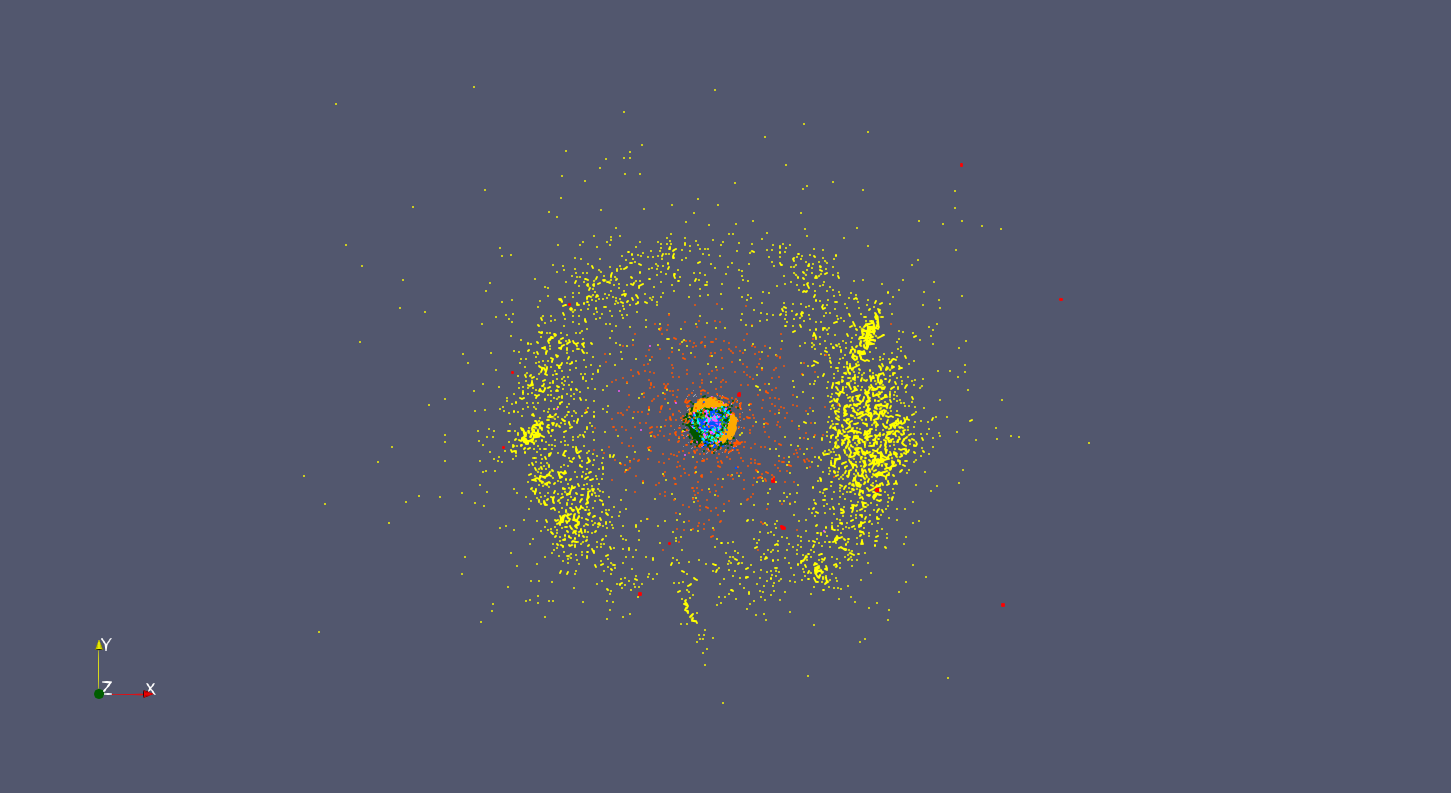
\includegraphics[width=\columnwidth]{figures/all_bodies_whole_system}
	            \caption{\setfontsize{10pt}Our solar system, including outer dwarf planets and TransNeptunian Objects.}
	        \end{figure}
	    \end{column}
	    \hspace*{2em}
	    \begin{column}{.45\linewidth}
	        \begin{figure}
	            \centering
	            \captionsetup{justification=centering}
	            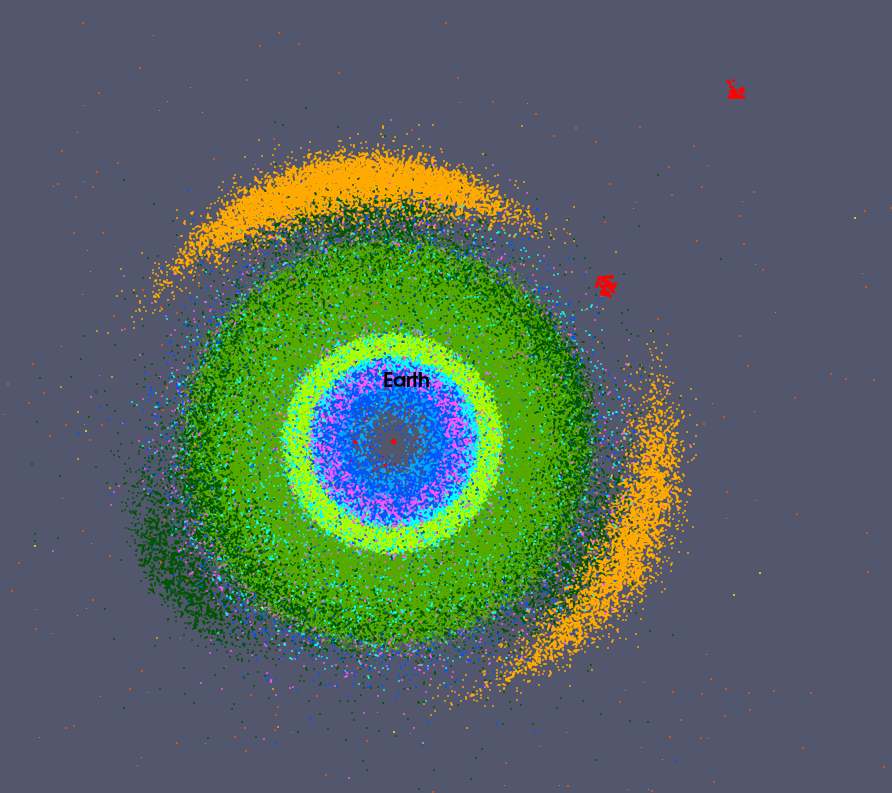
\includegraphics[width=.9\columnwidth]{figures/all_bodies_inner_system}
	            \caption{\setfontsize{10pt}Our solar system zoomed in to Jupiter and the main asteroid belt, Earth highlighted.}
	        \end{figure}
	    \end{column}
	\end{columns}
\end{frame}
%%%%%%%%%%%%%%%%%%%%%%%%%%%%%%%%%%%%%%%%%%%%%%%%%%%%%%%%%%%%%%%%%%%%

%%%%%%%%%%%%%%%%%%%%%%%%%%%%%%%%%%%%%%%%%%%%%%%%%%%%%%%%%%%%%%%%%%%%
\begin{frame}[fragile, c]
  \frametitle{Phase 1: Goal}
  \vspace*{-1em}
  \begin{center}
      Simulation of our solar system: planets, dwarf planets, moons, and asteroids \\(larger than \SI{10}{\kilo\meter}).\\[0.5em]

      \animategraphics[autoplay,loop,controls,width=.76\linewidth]{12}{figures/animation/output-}{0}{253}
  \end{center}
\end{frame}
%%%%%%%%%%%%%%%%%%%%%%%%%%%%%%%%%%%%%%%%%%%%%%%%%%%%%%%%%%%%%%%%%%%%

%%%%%%%%%%%%%%%%%%%%%%%%%%%%%%%%%%%%%%%%%%%%%%%%%%%%%%%%%%%%%%%%%%%%
\begin{frame}[fragile, c]
  \frametitle{Theory: Basic Idea of N-Body Simulations}
  The goal of an n-body simulation is to establish equations of motion for each body.

  \begin{center}
  \vspace*{-1em}
  \begin{tikzpicture}
  \coordinate (origo) at (0,0);
  \node[below=0.1 of origo] {$(0, 0, 0)$};

  % body 1
  \node[shading=ball,circle,minimum size=0.5cm,ball color=ForestGreen!80!white] at (5,5) (m1) {$m_1$};
  \draw [dotted,->] (origo) -- (m1) node[midway,sloped,below] {$\vec{r}_1$};
  \draw [dashed,thick,->,ForestGreen] (m1) -- ++(-1,1)  node[midway,sloped,above] {$\vec{v}_1$};
  \draw [dashed,thick,->,NavyBlue] (m1) -- ++(-0.8,-0.2) node[sloped,near end,anchor=east] {$\vec{a}_{1,2}$};
  \draw [dashed,thick,->,orange] (m1) -- ++(0.4,-0.6) node[sloped,near end,anchor=west] {$\vec{a}_{1,3}$};
  \draw [dashed,->,NavyBlue!60] (m1) ++(-1,1)  --  ++(-0.8,-0.2);
  \draw [dashed,->,orange!60] (m1) ++(-1.8,0.8)  --  ++(0.4,-0.6);
  \draw [very thick,->,red] (m1)   --  ++(-1.4,0.2);

  % body 2
  \node[shading=ball,circle,minimum size=0.5cm,ball color=NavyBlue!80!white] at (-3,3) (m2) {$m_2$};
  \draw [dotted,->] (origo) -- (m2) node[midway,sloped,below] {$\vec{r}_2$};
  \draw [dashed,thick,->,NavyBlue] (m2) -- ++(1,1.3)  node[midway,sloped,above] {$\vec{v}_2$};
  \draw [dashed,thick,->,ForestGreen] (m2) -- ++(0.8,0.2) node[sloped,near end,anchor=west] {$\vec{a}_{2,1}$};
  \draw [dashed,thick,->,orange] (m2) -- ++(1,-0.1) node[sloped,near end,anchor=west] {$\vec{a}_{2,3}$};
  \draw [dashed,->,ForestGreen!60] (m2)++(1,1.3) -- ++(0.8,0.2);
  \draw [dashed,->,orange!60] (m2)++(1.8,1.5) -- ++(1,-0.1);
  \draw [very thick,->,red] (m2) -- ++(2.8,1.4);

  % body 3
  \node[shading=ball,circle,minimum size=0.5cm,ball color=orange!80!white] at (7,2) (m3) {$m_3$};
  \draw [dotted,->] (origo) -- (m3) node[midway,sloped,below] {$\vec{r}_3$};
  \draw [dashed,thick,->,orange] (m3) -- ++(0.8,0.9)  node[midway,sloped,above] {$\vec{v}_3$};
  \draw [dashed,thick,->,ForestGreen] (m3) -- ++(-0.4,0.6) node[sloped,near end, anchor=east] {$\vec{a}_{3,1}$};
  \draw [dashed,thick,->,NavyBlue] (m3) -- ++(-1,0.1) node[sloped, near end, anchor=east] {$\vec{a}_{3,2}$};
  \draw [dashed,->,ForestGreen!60] (m3)++(0.8,0.9) -- ++(-0.4,0.6);
  \draw [dashed,->,NavyBlue!60] (m3)++(0.4,1.5) --  ++(-1,0.1);
  \draw [very thick,->,red] (m3) -- ++(-0.6,1.6);
  \end{tikzpicture}
  \end{center}
\end{frame}
%%%%%%%%%%%%%%%%%%%%%%%%%%%%%%%%%%%%%%%%%%%%%%%%%%%%%%%%%%%%%%%%%%%%

%%%%%%%%%%%%%%%%%%%%%%%%%%%%%%%%%%%%%%%%%%%%%%%%%%%%%%%%%%%%%%%%%%%%
\begin{frame}[fragile]
  \frametitle{Theory: Naive Formulation of an N-Body Simulation Problem}
  Each body $i$ with its mass $m_i$ and position vector $\vec{r}_i$ experiences the force $\vec{a}_i$ from all other bodies according to Newton's law of universal gravitation:
  \begin{equation*}
    \vec{a}_i = \sum\limits_{i \neq j} G m_j \frac{\vec{r}_j - \vec{r}_i}{(\norm{\vec{r}_j - \vec{r}_i}_2^2 + \epsilon^2)^\frac{3}{2}}
  \end{equation*}
  \pause
  \vfill
  \begin{itemize}
    \item gravitational constant: $G = \num{6.67430e-11}\frac{\text{m}^3}{\text{kg} \cdot \text{s}^2}$
    \item The physical units of $G$ do not reflect the units used in the data sets.
    \item softening factor: $\epsilon = \num{1e-11}$ to prevent collisions between two bodies
    \item $\norm{}_2^2$: squared Euclidean distance
  \end{itemize}
\end{frame}
%%%%%%%%%%%%%%%%%%%%%%%%%%%%%%%%%%%%%%%%%%%%%%%%%%%%%%%%%%%%%%%%%%%%

%%%%%%%%%%%%%%%%%%%%%%%%%%%%%%%%%%%%%%%%%%%%%%%%%%%%%%%%%%%%%%%%%%%%
\begin{frame}[fragile, label={phase1_requirements}]
  \frametitle{Phase 1: Requirements - Scenario 1}
  Simulating our solar system with the provided planets and moons as well as all asteroids with a \textbf{given} \texttt{diameter} and \texttt{albedo} and where the \textbf{main-belt asteroids} (\texttt{MBA}) are further constraint with a diameter \textbf{greater or equal} than \SI{10}{\kilo\meter} must not take longer than $\SI{1}{\hour}$ on our target system \texttt{simcl1} using $4$ compute nodes:
  \begin{center}
    \setfontsize{6.8pt}
    \mintinline{text}{srun --exclusive -N 4 ./simulate --file scenario1.csv --dt 1h --t_end 12y --vs 2d --vs_dir sim_s1 --theta 1.05}
    \begin{figure}
        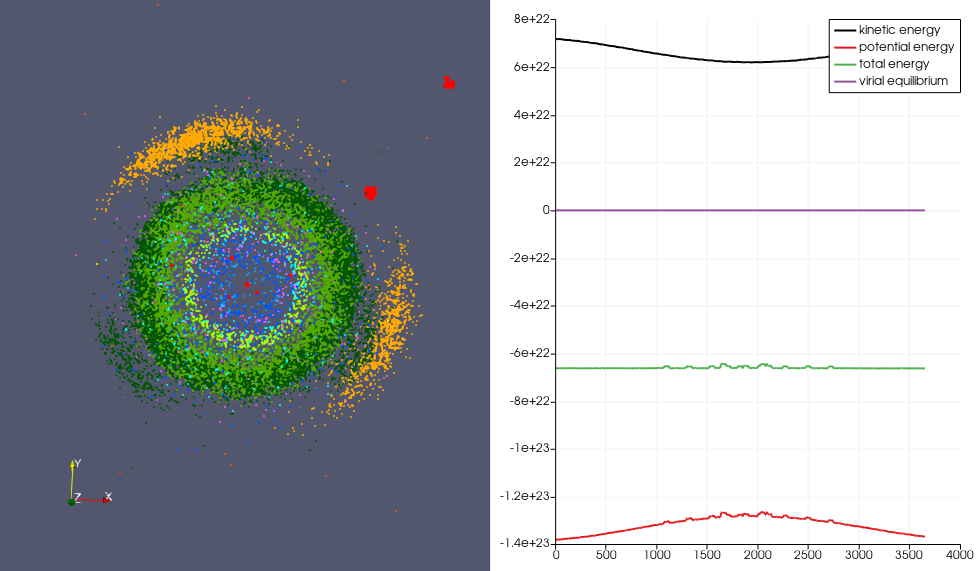
\includegraphics[width=.4\textwidth]{figures/scenario1_result.png}
        \caption{Simulation result of the inner solar system with different colors for the different orbit classes after \num{105192} time steps with \num{19054} bodies.}
    \end{figure}
  \end{center}
\end{frame}
%%%%%%%%%%%%%%%%%%%%%%%%%%%%%%%%%%%%%%%%%%%%%%%%%%%%%%%%%%%%%%%%%%%%

%%%%%%%%%%%%%%%%%%%%%%%%%%%%%%%%%%%%%%%%%%%%%%%%%%%%%%%%%%%%%%%%%%%%
\begin{frame}[fragile]
  \frametitle{Phase 1: Requirements - Scenario 2}
  This time you have \SI{30}{\minute} and again $4$ compute nodes. Try to simulate as many planets, moons, and asteroids as possible for one Earth year!
  \begin{center}
    \setfontsize{6.8pt}
    \mintinline{text}{srun --exclusive -N 4 ./simulate --file scenario2.csv --dt 1h --t_end 1y --vs 7d --vs_dir sim_s2 --theta 1.05} \\[.75em]

    \begin{figure}
        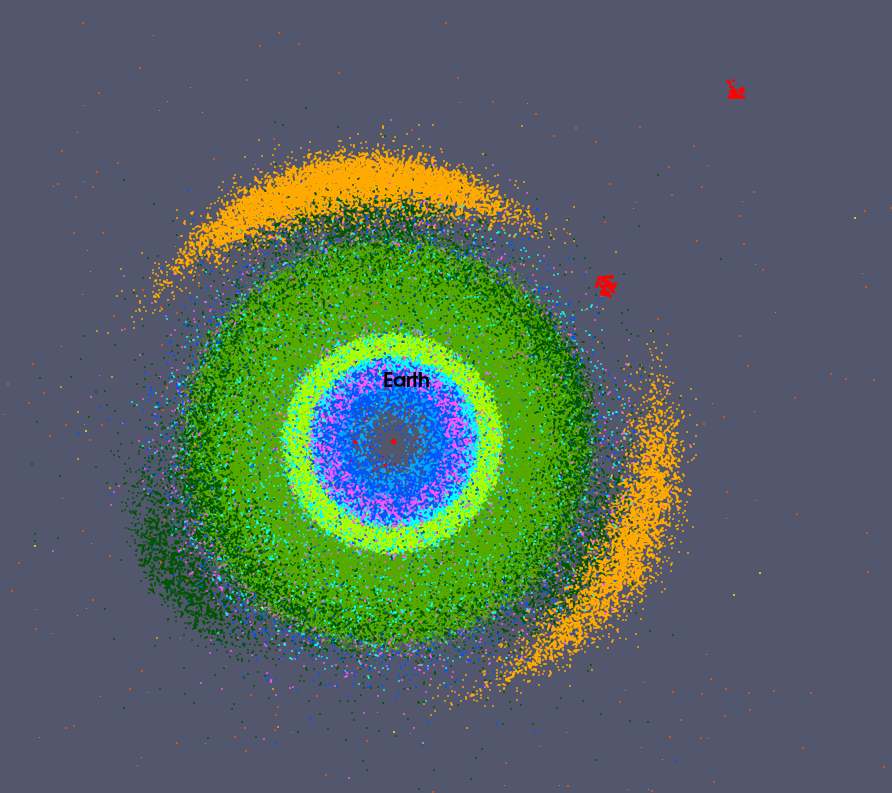
\includegraphics[width=.3\textwidth]{figures/all_bodies_inner_system}
        \caption{Example initial state with \num{1216869} bodies (approximately the maximum number of asteroids in NASA JPL's Small-Body Database).}
    \end{figure}
  \end{center}
\end{frame}
%%%%%%%%%%%%%%%%%%%%%%%%%%%%%%%%%%%%%%%%%%%%%%%%%%%%%%%%%%%%%%%%%%%%

%%%%%%%%%%%%%%%%%%%%%%%%%%%%%%%%%%%%%%%%%%%%%%%%%%%%%%%%%%%%%%%%%%%%
\begin{frame}
    \frametitle{Phase 1: Simulation Data}
    \begin{itemize}
        \item The data sets containing the planets and moons as well as the asteroids for scenario 1 can be found in \link{\urlIliasData}{ILIAS}:
        \item For scenario 2 additional asteroid data can be queried using NASA Jet Propulsion Laboratory's (JPL) \link{https://ssd.jpl.nasa.gov/tools/sbdb_query.html}{Small-Body Database}.
        \item Be aware that some bodies may appear multiple times (e.g., Pluto and its moons) and you have to take care that these bodies are only used once in the actual simulation!

        \item \textbf{Note:} all data is given using the Keplerian orbital elements that must first be converted to Cartesian state vectors.

        \item \textbf{Attention:} The Sun/Sol (with the reference mass \SI{1.98847e30}{\kilo\gram} and epoch $2451544.5$ JD) must always be \textbf{manually} added at the coordinate's origin since it is impossible to specify its orbital elements with respect to itself.

        \item All data must be saved and processed using double precision (FP64, \mintinline{c++}{double}) floating point types.
    \end{itemize}
\end{frame}
%%%%%%%%%%%%%%%%%%%%%%%%%%%%%%%%%%%%%%%%%%%%%%%%%%%%%%%%%%%%%%%%%%%%

%%%%%%%%%%%%%%%%%%%%%%%%%%%%%%%%%%%%%%%%%%%%%%%%%%%%%%%%%%%%%%%%%%%%
\begin{frame}[fragile]
  \frametitle{Phase 1: Submission - \dateDeadlinePhaseOne}
  \begin{itemize}
      \item Submission via \link{\urlIliasSubmissionPhaseOne}{ILIAS}.
      \item Scenario 1: animation of the 3D simulation with a reasonable temporal resolution.
      \item Scenario 2: your custom data set file; the name should contain the number of used bodies.
      \item Scenario 1 \& 2: image of the last time step created via ParaView including an energy plot (kinetic, potential, and total energies) and \texttt{scenario1/2\_save.csv} files with the end states (name, mass, positions, velocities) of the simulations.
      \item The ParaView specific \texttt{.pvd} and \texttt{.vtp} files must \textbf{not} be submitted!
      \item Diagrams with explanations regarding the runtimes (see next slide).
      \item One file, \texttt{submission.sh}, containing the following information (\mintinline{bash}{${}} replaced):
      \begin{minted}[fontsize=\footnotesize]{bash}
#!/bin/sh
git clone ${REPOSITORY_URL} ${GROUP_NAME}
cd ${GROUP_NAME} || exit
git checkout ${COMMIT_HASH}
      \end{minted}

      The commit must contain the code to be evaluated as well as a \texttt{README.md} file describing all necessary steps to build and run your code.

%   \textbf{Note:} it may be more convenient to create a separate git tag for your submission.
  \end{itemize}
\end{frame}
%%%%%%%%%%%%%%%%%%%%%%%%%%%%%%%%%%%%%%%%%%%%%%%%%%%%%%%%%%%%%%%%%%%%

%%%%%%%%%%%%%%%%%%%%%%%%%%%%%%%%%%%%%%%%%%%%%%%%%%%%%%%%%%%%%%%%%%%%
\begin{frame}[fragile]
  \frametitle{Phase 1: Performance Analysis}
  \begin{itemize}
      \item Diagram of the runtimes of the code fixing the number of MPI nodes and OpenMP threads and using different numbers of bodies.
      \item Diagram of the runtimes of the code fixing the number of MPI nodes and varying the number of OpenMP threads (e.g., via \mintinline{bash}{export OMP_NUM_THREADS=N}) for a fixed problem size.
      \item Diagram of the runtimes of the code fixing the number of OpenMP threads and varying the number of MPI nodes for a fixed problem size.
      \item Diagram displaying the runtime and the summed up distances to a very small $\theta$ using different values for $\theta$.
      \item Additional: each diagram must contain a possible \textbf{explanation} for the displayed behavior!
      \item \textbf{Note}: use suitable scenarios for all diagrams.
  \end{itemize}
\end{frame}
%%%%%%%%%%%%%%%%%%%%%%%%%%%%%%%%%%%%%%%%%%%%%%%%%%%%%%%%%%%%%%%%%%%%

%%%%%%%%%%%%%%%%%%%%%%%%%%%%%%%%%%%%%%%%%%%%%%%%%%%%%%%%%%%%%%%%%%%%
\begin{frame}[fragile]
  \frametitle{Phase 1: Competitions}
  Two competitions:
  \begin{itemize}
      \item Which group produces the prettiest simulation animation for scenario 1?
      \begin{itemize}
          \item How to best display the vastly different body sizes in ParaView?
          \item Added body textures?
          \item Camera movement?
      \end{itemize}
      \item Which group can simulate the most bodies in the available time? (scenario 2)
      \begin{itemize}
          \item Add your runtime and number of bodies to the \link{\urlNextcloud}{Nextcloud table}% using the password \texttt{\passwordNextcloud}.
          \item At the end of phase 1, the runtimes and number of bodies will be verified by us.
          \item Real simulation without tricks (e.g., it is \textbf{not} allowed to simply output pre-calculated time steps!).
      \end{itemize}
  \end{itemize}
    \vfill
  \itFollows{The winners of each competition will receive a small reward!}
\end{frame}
%%%%%%%%%%%%%%%%%%%%%%%%%%%%%%%%%%%%%%%%%%%%%%%%%%%%%%%%%%%%%%%%%%%%

\section*{Phase 2}
%%%%%%%%%%%%%%%%%%%%%%%%%%%%%%%%%%%%%%%%%%%%%%%%%%%%%%%%%%%%%%%%%%%%
\begin{frame}
	\frametitle{Phase 2: Goal}
    \vspace*{-0.2cm}
    \visible<2->{
    \begin{tikzpicture}[overlay]
        \node at (2.9, -.55) {
\includegraphics[width=2.85cm]{figures/phase_2_intro/HPX_STELLAR_blue.png}\tiny[1]};

        \begin{scope}[scale=.8, shift={(0, -1.5)}]
            \node (gpu) at (2, -1.5) {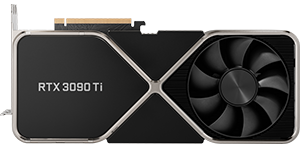
\includegraphics[width=3.5cm]{figures/phase_2_intro/nvidia-geforce-rtx-3090-ti.png}\tiny[2]};

            \node (cuda) at (0.5, -3.75) {
\includegraphics[width=1.2cm]{figures/phase_2_intro/Nvidia_CUDA_Logo.jpg}};
            \node (sycl) at (3.5, -3.75) {
\includegraphics[width=1.5cm]{figures/phase_2_intro/sycl_logo.png}};
            \node (opencl) at (2, -4.5) {
\includegraphics[width=1.5cm]{figures/phase_2_intro/OpenCL_logo.svg.png}};

            \draw[dashed, -latex] (gpu) -- (cuda);
            \draw[dashed, -latex] (gpu) -- (sycl);
            \draw[dashed, -latex] (gpu) -- (opencl);
        \end{scope}
        \node at (11.75, 0) {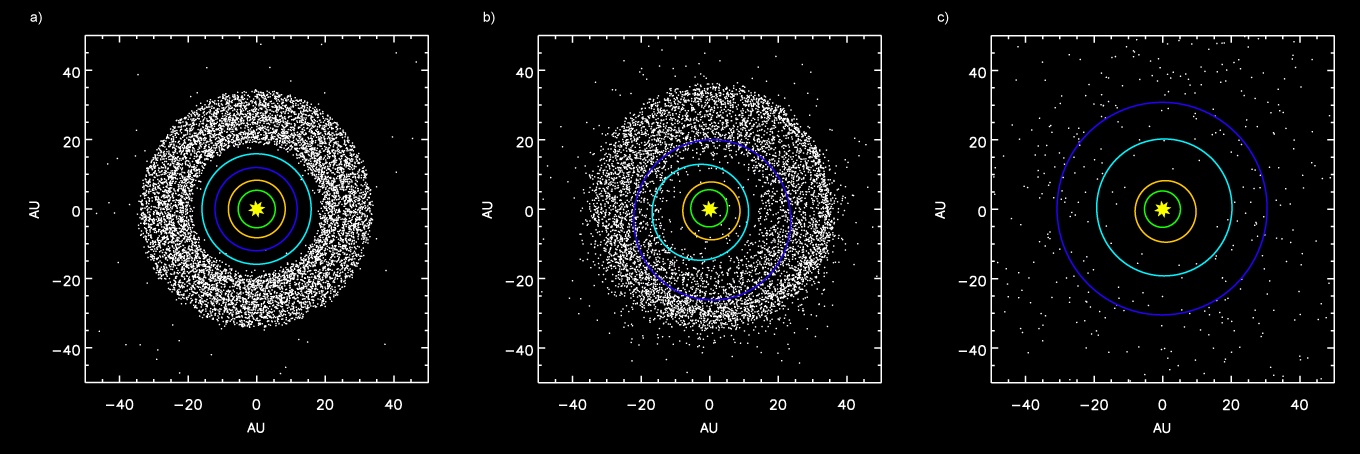
\includegraphics[width=6cm]{figures/phase_2_intro/nice_model.png}\,\tiny[3]};
        \node at (11.5, -3.25) {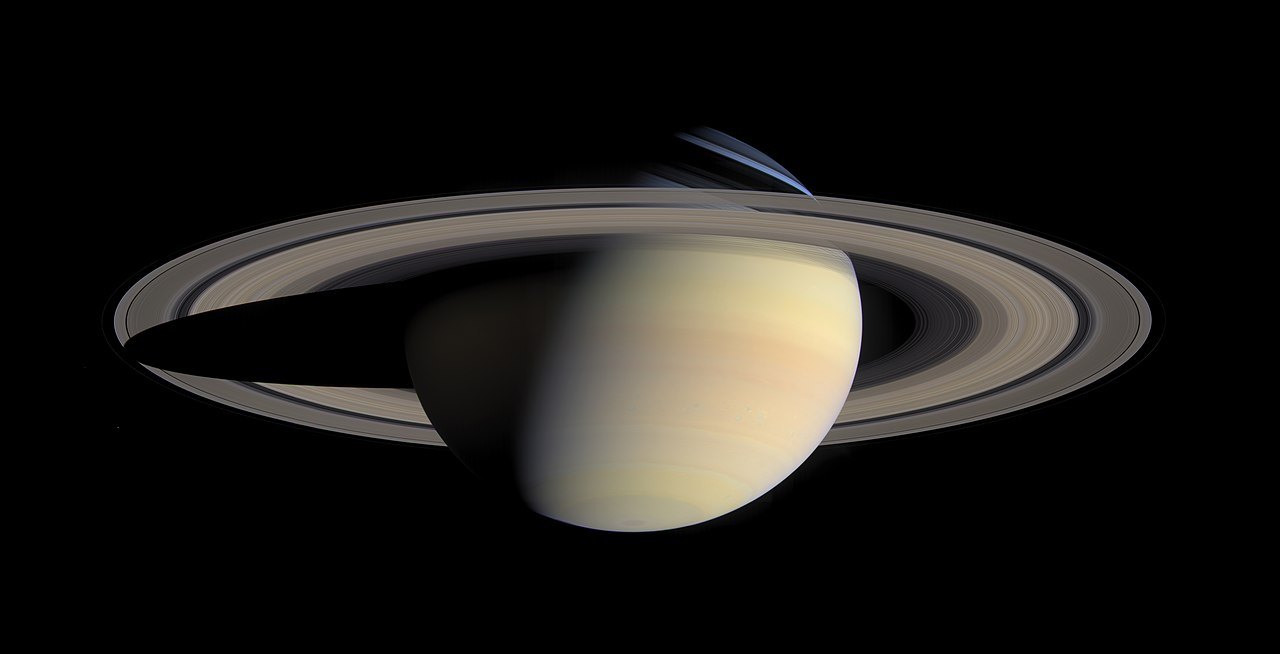
\includegraphics[width=5cm]{figures/phase_2_intro/1280px-Saturn_from_Cassini_Orbiter_(2004-10-06).jpeg}\,\tiny[4]};
    \end{tikzpicture}
    }

	\vspace*{-2.5cm}
	\begin{center}
	    \bfseries \setfontsize{150pt}%
	    ?
	\end{center}


	\btVFill
	\centering
    \vspace*{3em}
	\DisplayRightArrow Everyone can do a custom project on his own based on the code of phase 1.
	\vspace{-.25em}
	\visible<2->{
    	\begin{flushleft}
        \tiny Image Sources: \\
    	\tiny [1]: \url{https://hpx-docs.stellar-group.org/latest/html/index.html} \\
    	\tiny [2]: \url{https://store.nvidia.com/de-de/geforce/store/?page=1&limit=9&locale=de-de} \\
    	\tiny [3]: \url{https://en.wikipedia.org/wiki/Nice_model} \\
    	\tiny [4]: \url{https://en.wikipedia.org/wiki/Saturn}
    	\end{flushleft}
	}
\end{frame}
%%%%%%%%%%%%%%%%%%%%%%%%%%%%%%%%%%%%%%%%%%%%%%%%%%%%%%%%%%%%%%%%%%%%

%%%%%%%%%%%%%%%%%%%%%%%%%%%%%%%%%%%%%%%%%%%%%%%%%%%%%%%%%%%%%%%%%%%%
\begin{frame}
	\frametitle{Phase 2: Goal}
	Extend your code of phase 1 by an individual project, possible examples are:
	\begin{itemize}
	    \item code acceleration using GPUs (e.g., via CUDA, OpenCL, Kokkos, or SYCL)
	    \item replacing MPI with another framework for distributed computing like HPX
	    \item add more physics (e.g., collision detection for simulating the Kessler syndrome)
	    \item implementing more efficient algorithms (e.g., Fast Multipole Methods)
	    \item lifting the simplification that every node saves all bodies \\
	    $\rightarrow$ each node only knows about a subset of all bodies (needs load balancing)
	    \item new simulation scenarios (e.g., close-up simulation of Saturn including its rings, the Oort Cloud with Nemesis, the Nice model, or the \enquote{galaxy far, far away})
	    \item $\dots$
	\end{itemize}
	\begin{center}
	    \textbf{Restrictions:} It must have something to do with our overall parallelism topic and it must be different from your group members' projects!
	\end{center}
	\btVFill
	\itFollows{Each project must be approved by us, i.e., simply send us an email with 2-3 sentences describing your idea before you start working on it.}
\end{frame}
%%%%%%%%%%%%%%%%%%%%%%%%%%%%%%%%%%%%%%%%%%%%%%%%%%%%%%%%%%%%%%%%%%%%

%%%%%%%%%%%%%%%%%%%%%%%%%%%%%%%%%%%%%%%%%%%%%%%%%%%%%%%%%%%%%%%%%%%%
\begin{frame}[fragile]
  \frametitle{Phase 2: Submission - \dateDeadlinePhaseTwo}
  \begin{itemize}
      \item Submission via \link{\urlIliasSubmissionPhaseTwo}{ILIAS}.
      \item A \texttt{submission.sh} file as for \hyperref[phase1_requirements]{phase 1} with adjusted placeholders and commit hash.
      \item A \texttt{.pdf} describing your project idea, implementation, and possible results on \textbf{at least} 5 pages excluding the title page and possible references
      \item All supplementary files for your individual project (e.g., simulation data sets for a new scenario or new runtime diagrams).
      \item The \link{\urlIliasLatexTemplate}{\LaTeX\xspace template} can be found in ILIAS.
  \end{itemize}
\end{frame}
%%%%%%%%%%%%%%%%%%%%%%%%%%%%%%%%%%%%%%%%%%%%%%%%%%%%%%%%%%%%%%%%%%%%

%%%%%%%%%%%%%%%%%%%%%%%%%%%%%%%%%%%%%%%%%%%%%%%%%%%%%%%%%%%%%%%%%%%%
\begin{frame}[fragile]
  \frametitle{Phase 2: Presentation - \dateFinal}
  \begin{itemize}
    \item $15$-$\SI{20}{\minute}$ presentation + $\SI{5}{\minute}$ Q\&A per student.
    \item The slides must be uploaded in \link{\urlIliasSubmissionFinal}{ILIAS}.
    \item Phase 2 will be the crucial part for your grade where this presentation is a major part of! The results from phase 1 play only a minor role in grading!
    \vspace*{1em}
    \item The slides should contain all your results of phase 2.
    \item They should also contain the problems you encountered during phase 2.
  \end{itemize}
\end{frame}
%%%%%%%%%%%%%%%%%%%%%%%%%%%%%%%%%%%%%%%%%%%%%%%%%%%%%%%%%%%%%%%%%%%%

\section*{General Remarks}
%%%%%%%%%%%%%%%%%%%%%%%%%%%%%%%%%%%%%%%%%%%%%%%%%%%%%%%%%%%%%%%%%%%%
\begin{frame}[fragile]
  \frametitle{General Submission Guidelines}
  \begin{itemize}
    \item For each phase \textbf{exactly} one \texttt{*.zip} or \texttt{*.tar.gz} archive must be uploaded to \link{\urlIliasCourse}{ILIAS} with the content corresponding to the respective phase.
    \item PhasePhasenumber followed by the family name (of all group members), e.g., \texttt{Phase1\_Name1\_Name2\_Name3.tar.gz}.
    \item Each file in the archive must contain the name (of \textbf{all} group members).
    \item The submission must be compilable and executable on a normal Linux command line on one of our machines, i.e., no IDE specific build scripts are allowed!
  \end{itemize}
\end{frame}
%%%%%%%%%%%%%%%%%%%%%%%%%%%%%%%%%%%%%%%%%%%%%%%%%%%%%%%%%%%%%%%%%%%%

%%%%%%%%%%%%%%%%%%%%%%%%%%%%%%%%%%%%%%%%%%%%%%%%%%%%%%%%%%%%%%%%%%%%
\begin{frame}
  \frametitle{GitLab}
  \begin{itemize}
    \item After applying for our hardware and receiving an account, this account can also be used to login to our \link{https://gitlab-sim.informatik.uni-stuttgart.de}{GitLab server}.
    \item For phase 1, you get one private repository per submission group, for phase 2, one fork of the phase 1 repository per student.
    \item Each repository \textbf{must} have one \texttt{README} file containing all necessary information on how to compile and execute your code.
    \item An \link{https://github.com/SCTeaching-NBody/LabCourse_Template}{example \texttt{C++ \& CMake} repository} with small MPI + OpenMP code snippets can also be found in our GitLab.
  \end{itemize}
\end{frame}
%%%%%%%%%%%%%%%%%%%%%%%%%%%%%%%%%%%%%%%%%%%%%%%%%%%%%%%%%%%%%%%%%%%%

%%%%%%%%%%%%%%%%%%%%%%%%%%%%%%%%%%%%%%%%%%%%%%%%%%%%%%%%%%%%%%%%%%%%
\begin{frame}{CI via GitLab}

\begin{itemize}
    \item You should at least have 10 useful test cases and a test coverage of at least \SI{80}{\percent}!
    \item Install a GitLab runner on your machine and register a runner for your repository/fork.
    \begin{itemize}
        \item \link{https://docs.gitlab.com/runner/install/}{Install instructions} for a GitLab runner.
        \item GitLab runner as docker service as shown in the \link{https://github.com/Simulation-Software-Engineering/Lecture-Material/blob/main/05_testing_and_ci/gitlab_ci_demo.md}{SSE lecture}.
        \item The runner should support the docker executor and should be able to run Linux images.
    \end{itemize}
    \item Add a GitLab pipeline status badge to the project that is based on your pipeline and the main branch.
\end{itemize}

If you cannot add such a runner on your machine, please email one of us with the registration token and your GitLab username. We will then add a runner to your repository.

\end{frame}
%%%%%%%%%%%%%%%%%%%%%%%%%%%%%%%%%%%%%%%%%%%%%%%%%%%%%%%%%%%%%%%%%%%%

%%%%%%%%%%%%%%%%%%%%%%%%%%%%%%%%%%%%%%%%%%%%%%%%%%%%%%%%%%%%%%%%%%%%
\begin{frame}[fragile]
  \frametitle{Allowed Software}
  \begin{itemize}
      \item You are allowed to use any third-party library that does \textbf{not} solve a significant part of your project (like converting the orbital elements to state vectors, performing the actual simulation, writing the ParaView output, etc.).
      \item If you are not sure if you are allowed to use a library, feel free to contact us via email or ILIAS.
      \item Utility libraries, however, are allowed and we recommend the usage of the following:
      \begin{itemize}
          \item any command line parser library (e.g., \link{https://github.com/jarro2783/cxxopts}{\texttt{cxxopts}})
          \item the \texttt{C++} formatting library \link{https://github.com/fmtlib/fmt}{\texttt{\{fmt\}}}
      \end{itemize}
      \item \textbf{Note:} you \textbf{must} provide installation instructions for every library you use! Or better use something like CMake's \mintinline{text}{FetchContent_Declare} to install it if possible automatically.
      \item Another way to install third-party libraries without the need for root privileges is \link{https://github.com/spack/spack}{\texttt{spack}}.
      \item Any \texttt{C++} standard from \texttt{C++17} and upwards is allowed.
  \end{itemize}
\end{frame}
%%%%%%%%%%%%%%%%%%%%%%%%%%%%%%%%%%%%%%%%%%%%%%%%%%%%%%%%%%%%%%%%%%%%

%%%%%%%%%%%%%%%%%%%%%%%%%%%%%%%%%%%%%%%%%%%%%%%%%%%%%%%%%%%%%%%%%%%%
\begin{frame}[fragile]
  \frametitle{General Recommendations and Remarks}
  \begin{itemize}
    \item Your simulation should include some sort of progress indication (e.g., a terminal output each \SI{10}{\percent} of the simulation).
    \item Use a \texttt{C++} IDE (e.g., Visual Studio (Code) or CLion) and their tools like profiler, debugger, auto-formatting, linter, etc.
    \item Use an automated build system, preferable \link{https://cmake.org/}{CMake}.
    \item Document your code (for you \textbf{and} for us!), e.g., via \link{https://doxygen.nl/}{Doxygen}.
    \item The installation and usage of your program as well as its verification should be as easy as possible.
    \item Test your program on our target Linux system \texttt{simcl1}.
    \item One of the main goals of this lab course is to encourage working independently, however, if questions arise, feel free to ask them in the \link{\urlIliasForumGeneral}{ILIAS forum}.
    \item The easiest way to determine the total runtime of your code is to use the Linux \mintinline{bash}{time} utility: \mintinline{bash}{time ./simulate --file data.csv --dt 1h --t_end 1y --vs 2d --theta 1.05}
    \item Start to work on phase 1 and phase 2 soon enough!
    \item Secret tip: MIT's \link{https://missing.csail.mit.edu/}{\enquote{The Missing Semester of Your CS Education}}
  \end{itemize}
\end{frame}
%%%%%%%%%%%%%%%%%%%%%%%%%%%%%%%%%%%%%%%%%%%%%%%%%%%%%%%%%%%%%%%%%%%%

%%%%%%%%%%%%%%%%%%%%%%%%%%%%%%%%%%%%%%%%%%%%%%%%%%%%%%%%%%%%%%%%%%%%
\begin{frame}[fragile]
	\frametitle{Time-Management Phase 1:}
	\begin{itemize}
		\item Think about a suitable time schedule: \textbf{when} should we implement \textbf{what}.
		\item For a successful Phase 1, we suggest the following rough schedule:
		\begin{description}
			%\setlength\itemsep{.4em}
			\item[1st week] project-setup, IO, and conversion from keplerian orbital elements to cartesian state vectors
			\item[2nd week] implement the naive approach to get familiar with the n-body problem (not needed for the final submission)
			\item
			\item[meeting]
			\item
			\item[3rd week] implement the Barnes-Hut algorithm
			\item[4th week] paralleize your implementation using MPI + OpenMP
			\item
			\item[meeting]
			\item
			\item[5th week] further optimize and benchmark your code
		\end{description}
	\end{itemize}
	
\end{frame}
%%%%%%%%%%%%%%%%%%%%%%%%%%%%%%%%%%%%%%%%%%%%%%%%%%%%%%%%%%%%%%%%%%%%

%%%%%%%%%%%%%%%%%%%%%%%%%%%%%%%%%%%%%%%%%%%%%%%%%%%%%%%%%%%%%%%%%%%%
\begin{frame}{On a Final Note}
    \begin{center}
        \Large\bfseries\itshape
        The simulation is greatly simplified!
    \end{center}
    \pause
    \vfill
    Many physical effects or properties are ignored or only roughly estimated:
    \begin{itemize}
        \item rotational forces, tidal forces, radiation, magnetic fields, etc.
        \item various value approximations, mainly for the asteroids' masses
        \item shape of the body (assumed to be spherical)
        \item $\dots$
    \end{itemize}
    \pause
    \vfill
    \itFollows{Nevertheless, it is good enough for a stable simulation of the whole of our solar system including the sun, planets, dwarf planets, moons, and major asteroids!}
\end{frame}
%%%%%%%%%%%%%%%%%%%%%%%%%%%%%%%%%%%%%%%%%%%%%%%%%%%%%%%%%%%%%%%%%%%%

%%%%%%%%%%%%%%%%%%%%%%%%%%%%%%%%%%%%%%%%%%%%%%%%%%%%%%%%%%%%%%%%%%%%
\begin{frame}[label={important_deadlines}]
  \frametitle{Important Dates and Deadlines}

  \begin{description}
    \item[\dateKickoffPhaseOne] Kick-off
    \item[\dateDeadlinePhaseZero] \textbf{Deadline Group Formation}
    \item[\dateDeadlinePhaseOneFirstMeeting] First Meeting Phase 1
    \item[\dateDeadlinePhaseOneSecondMeeting] Second Meeting Phase 1
    \item[\dateDeadlinePhaseOne] \textbf{Deadline Phase 1}
    \item[\dateDeadlinePhaseTwoFirstMeeting] First Meeting Phase 2
    \item[\dateDeadlinePhaseTwoSecondMeeting] Second Meeting Phase 2
    \item[\dateDeadlinePhaseTwo] \textbf{Deadline Phase 2}
    \item[\dateFinal] Final Presentations% (possibly on more than one day)
  \end{description}
  \vfill
  \itFollows{\textbf{Do not} forget to register for our lab course in \link{https://campus.uni-stuttgart.de}{C@MPUS}!}
\end{frame}
%%%%%%%%%%%%%%%%%%%%%%%%%%%%%%%%%%%%%%%%%%%%%%%%%%%%%%%%%%%%%%%%%%%%
